\documentclass[border=10pt]{standalone}
\usepackage[svgnames]{xcolor}
\usepackage{amsmath}
\usepackage{pgfplots}
\pgfplotsset{compat=newest}
\usepackage[sfdefault]{FiraSans}
\usepackage{FiraMono}
\renewcommand*\familydefault{\sfdefault}
\begin{document}
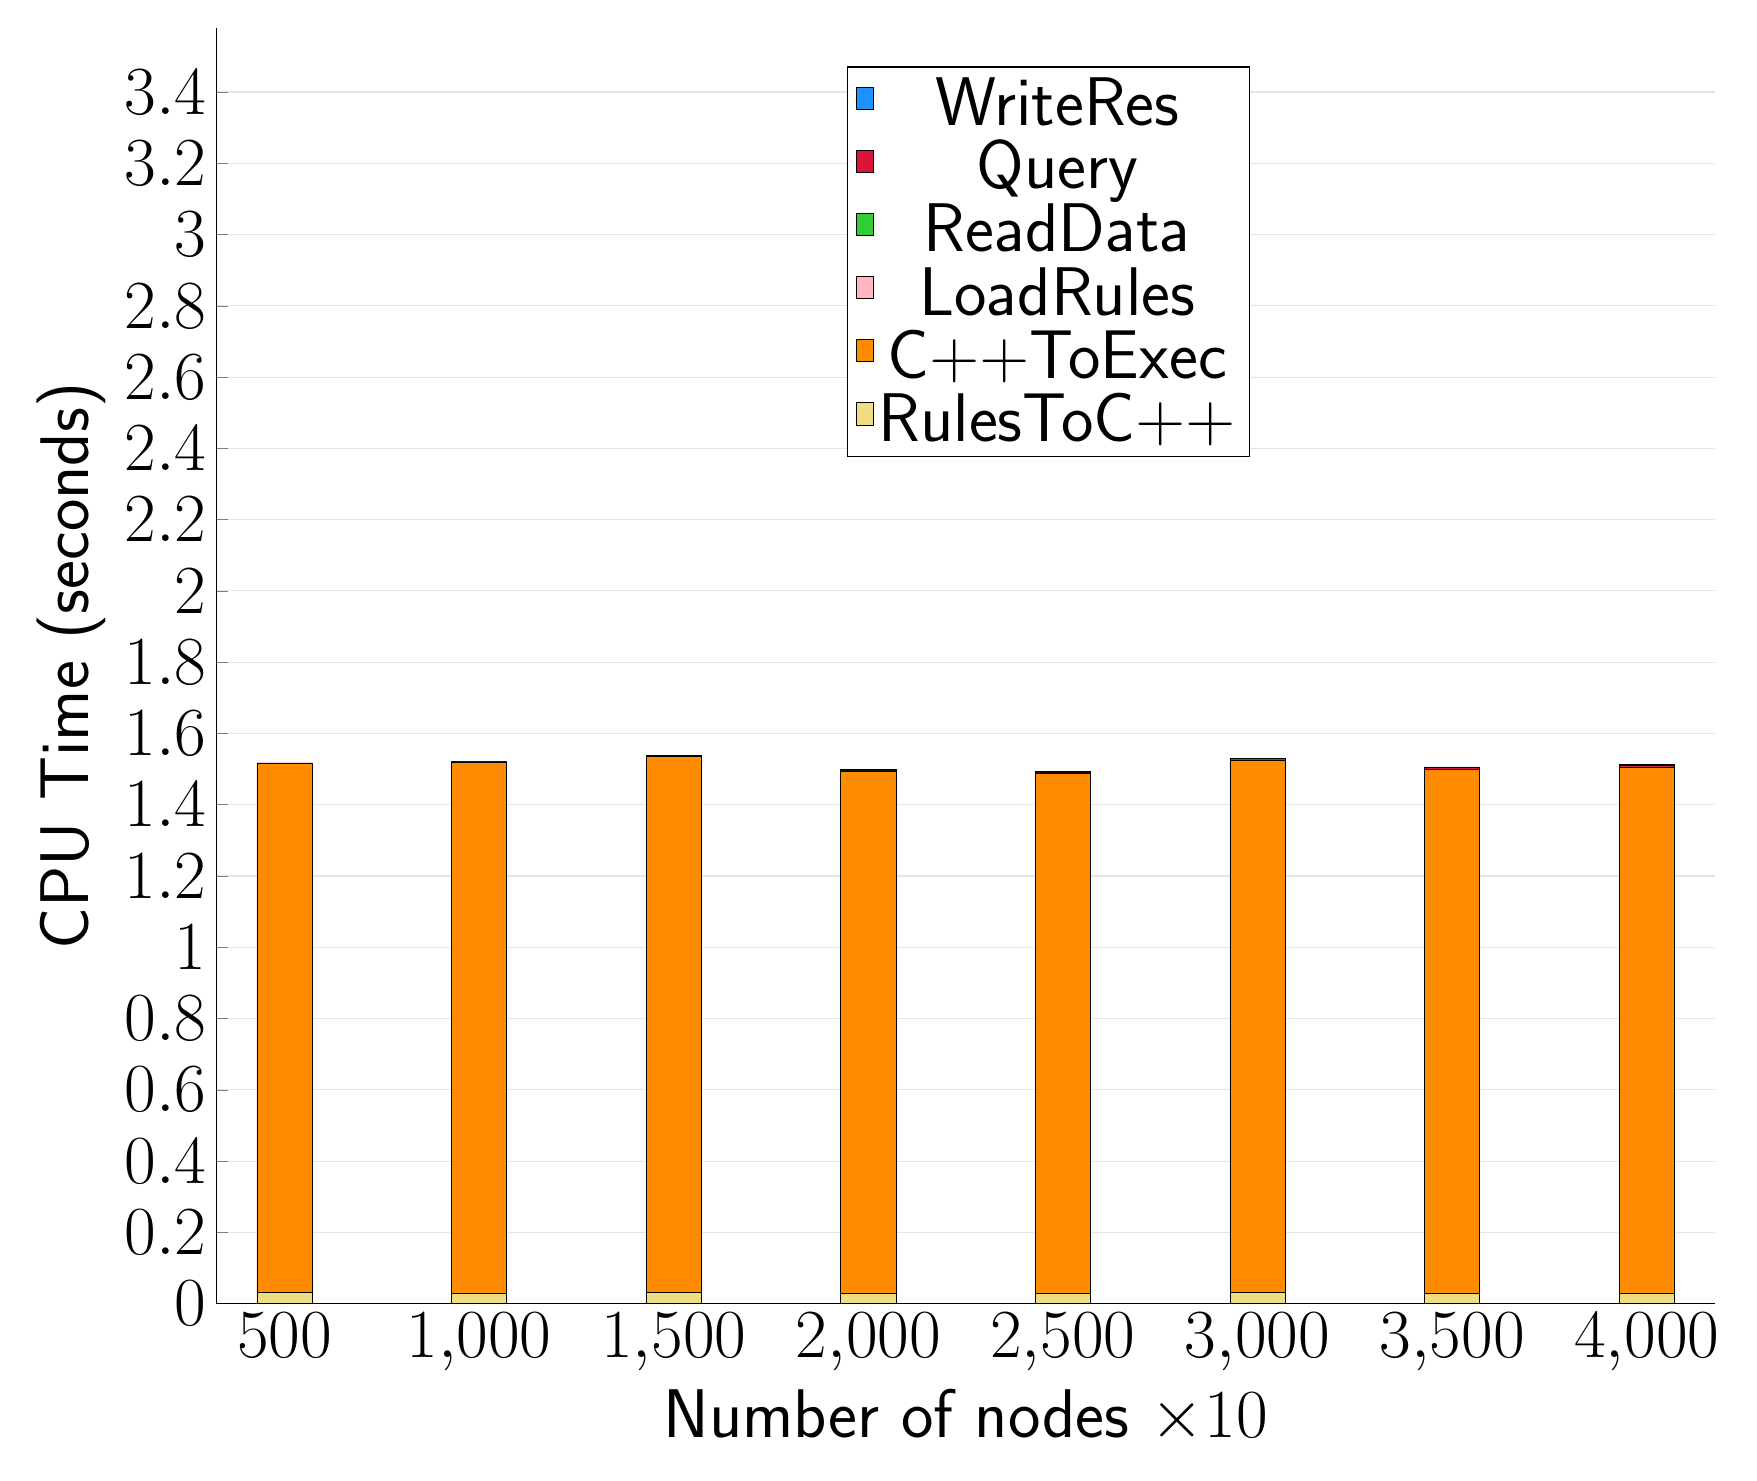
\begin{tikzpicture}
\begin{axis}[
   ybar stacked,
   width=1.7\textwidth,
   bar width=0.7cm,
   ymajorgrids, tick align=inside,
   major grid style={draw=gray!20},
   xtick=data,
   ymin=0, ymax=3.579,
   axis x line*=bottom,
   axis y line*=left,
   enlarge x limits=0.05,
   legend style={
       at={(0.69, 0.97)},
       anchor=north east,
       legend columns=1,
       font=\Huge,
   },
   ylabel={CPU Time (seconds)},
   xlabel={Number of nodes $\times 10$},
   label style={font=\Huge},
   tick label style={font=\Huge},
]
\addlegendimage{fill=DodgerBlue, draw=black, line width=0.2pt}
\addlegendentry{WriteRes}
\addlegendimage{fill=Crimson, draw=black, line width=0.2pt}
\addlegendentry{Query}
\addlegendimage{fill=LimeGreen, draw=black, line width=0.2pt}
\addlegendentry{ReadData}
\addlegendimage{fill=LightPink, draw=black, line width=0.2pt}
\addlegendentry{LoadRules}
\addlegendimage{fill=DarkOrange, draw=black, line width=0.2pt}
\addlegendentry{C++ToExec}
\addlegendimage{fill=LightGoldenrod, draw=black, line width=0.2pt}
\addlegendentry{RulesToC++}
\addplot +[fill=LightGoldenrod, draw=black, line width=0.2pt] coordinates {
(500, 0.030999999999999993)
(1000, 0.030000000000000006)
(1500, 0.030999999999999993)
(2000, 0.030000000000000006)
(2500, 0.030000000000000006)
(3000, 0.030999999999999993)
(3500, 0.030000000000000006)
(4000, 0.030000000000000006)
};
\addplot +[fill=DarkOrange, draw=black, line width=0.2pt] coordinates {
(500, 1.485)
(1000, 1.4900000000000002)
(1500, 1.5050000000000001)
(2000, 1.464)
(2500, 1.459)
(3000, 1.494)
(3500, 1.4689999999999999)
(4000, 1.4750000000000003)
};
\addplot +[fill=LightPink, draw=black, line width=0.2pt] coordinates {
(500, 0.0)
(1000, 0.0)
(1500, 0.0)
(2000, 1.01e-05)
(2500, 0.0)
(3000, 1e-05)
(3500, 1.06e-05)
(4000, 0.0)
};
\addplot +[fill=LimeGreen, draw=black, line width=0.2pt] coordinates {
(500, 0.0004075)
(1000, 0.0005214000000000001)
(1500, 0.000622)
(2000, 0.000753)
(2500, 0.0008423999999999999)
(3000, 0.0009411999999999999)
(3500, 0.0010289)
(4000, 0.0011713000000000001)
};
\addplot +[fill=Crimson, draw=black, line width=0.2pt] coordinates {
(500, 0.0006563)
(1000, 0.0012230000000000003)
(1500, 0.0017849)
(2000, 0.0024925000000000004)
(2500, 0.0031332)
(3000, 0.0035185999999999993)
(3500, 0.0041648)
(4000, 0.0048505)
};
\addplot +[fill=DodgerBlue, draw=black, line width=0.2pt] coordinates {
(500, 0.00044479999999999986)
(1000, 0.0006732)
(1500, 0.0009117)
(2000, 0.0011207)
(2500, 0.001363)
(3000, 0.0014960999999999998)
(3500, 0.0017222000000000001)
(4000, 0.0019084)
};
\end{axis}
\end{tikzpicture}

\end{document}
